% !TEX root = ../paper.tex

As a declarative language, the abstract syntax tree (AST) of a SQL statement acts as a proxy for the intent of the query author. We thus argue that structural similarity is a meaningful metric for query similarity.
For instance, we can group a query $Q$ with other queries that have nearly (or completely) the same AST as $Q$.
This structural definition of intent has seen substantial use already, particularly in the translation of natural language queries into SQL~\cite{li2015NLPI}.  

\begin{figure}[h!]
\centering
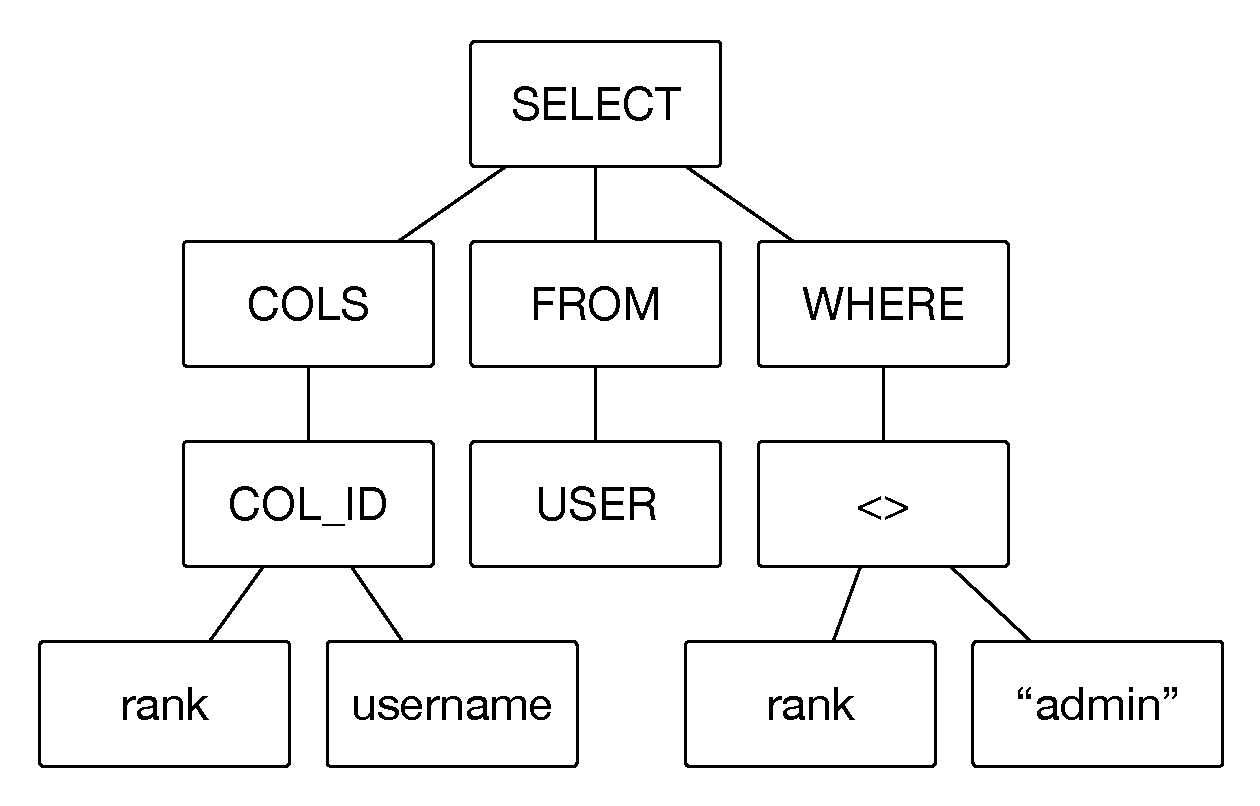
\includegraphics[width=6cm]{graphics/ast2}
\caption{An abstract syntax tree of query \texttt{SELECT rank, username FROM USER WHERE  rank <> "admin"}.}
\label{fig:exampleAST}
\end{figure}

As explained in Section~\ref{sec:background}, existing similarity metrics mainly utilize the columns from specific parts of the query; making use of the combination of projection, selection, joins, or group by items. However, we claim that having the same set of items does not necessarily imply that these queries have similar intents, even when they operate on similar domains. Consider the following example:

\begin{example} Queries accessing same columns
\label{ex:samecolumns}
\begin{enumerate}
\item\begin{verbatim}SELECT username FROM USER
WHERE  rank = "admin"\end{verbatim}
\item\begin{verbatim}SELECT DISTINCT COUNT(username), rank FROM USER
WHERE rank <> "admin"
GROUP BY rank
\end{verbatim}
\end{enumerate}
\end{example}

For the remainder of this paper, we will use $Q$ to denote both the query itself as well as its tree encoding.
The queries $Q_1$ and $Q_2$ in Example~\ref{ex:samecolumns} share the same set of columns; \texttt{username}, and \texttt{rank}. Nevertheless, it is obvious that $Q_1$ aims to list all usernames with admin rank, while $Q_2$ intends to count the number of users for every rank except the ones with admin rank. While having overlapping sets of items indicates a potential similarity, the intent behind these queries are completely different. This problem can easily be solved if we utilize the query ASTs. The AST of \texttt{WHERE} clause expressions of both queries can be seen on Figure~\ref{fig:subtrees}.

\begin{figure}[h!]
\captionsetup[subfigure]{justification=centering}
    \centering
    \begin{subfigure}[b]{0.22\textwidth}
        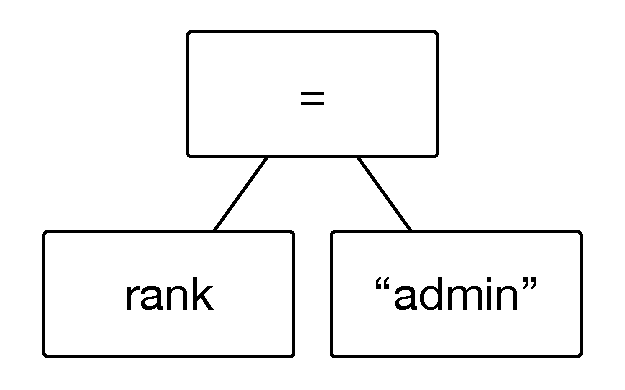
\includegraphics[width=\textwidth]{graphics/ex_subtree2}
        \caption{The subtree of expression $Q_1$:\texttt{rank = "admin"}}
        \label{fig:subtree1}
    \end{subfigure}
    ~ 
    \begin{subfigure}[b]{0.22\textwidth}
        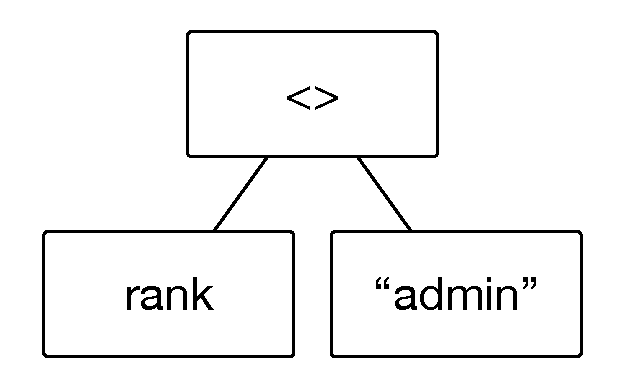
\includegraphics[width=\textwidth]{graphics/ex_subtree1}
        \caption{The subtree of expression $Q_2$:\texttt{rank <> "admin"}}
        \label{fig:subtree2}
    \end{subfigure}
    \caption{Two example subtrees}
    \label{fig:subtrees}
\end{figure}

According to the metrics surveyed in Section~\ref{sec:background}, the expressions \texttt{rank = "admin"} and \texttt{rank <> "admin"} are the same, because the only grammar item they would consider while calculating pairwise similarity is the column \texttt{rank}. We, on the other hand, argue that we need to consider all items and all expressions. Table~\ref{table:features} shows all features we can utilize. 
%Hence, our feature set is  Feature 1: \textit{rank}, Feature 2: \textit{=}, Feature 3: \textit{<>}, Feature 4: \textit{``admin''}, Feature 5: \textit{rank = ``admin''} and Feature 6: \textit{rank <> ``admin''}.

\begin{table}[h!]
\centering
\caption{Feature set of $Q_1$ and $Q_2$}
\label{table:features}
    \begin{tabular}{|| c | c ||}
    \hline
    \textbf{Feature} & \textbf{Item} \\ \hline
    1 & \textit{rank} \\ \hline
    2 & \textit{=} \\ \hline
    3 & \textit{<>} \\ \hline
    4 & \textit{``admin''} \\ \hline
    5 & \textit{rank = ``admin''} \\ \hline
    6 & \textit{rank <> ``admin''} \\
    \hline
    \end{tabular}
\end{table}

When we construct feature vectors \textbf{$v_1$} and \textbf{$v_2$} by counting the appearance of each feature in $Q_1$ and $Q_2$ respectively, we end up with the vectors listed in Table~\ref{tab:vectors}.

\begin{table}[!htbp]
\centering
\begin{tabular}{|c|c|c|c|c|c|c|}
\hline
\multirow{2}{*}{\textbf{Vectors}} & \multicolumn{6}{c|}{\textbf{Features}}                                      \\ \cline{2-7} 
                                  & \textbf{1} & \textbf{2} & \textbf{3} & \textbf{4} & \textbf{5} & \textbf{6} \\ \hline
\textbf{$v_1$}                       & 1          & 1          & 0          & 1          & 1          & 0          \\ \hline
\textbf{$v_2$}                       & 1          & 0          & 1          & 1          & 0          & 1          \\ \hline
\end{tabular}
\caption{Feature vectors constructed for queries $Q_1$ and $Q_2$ (See Example~\ref{ex:samecolumns}).}
\label{tab:vectors}
\end{table}
Pairwise similarity between the two queries can now be computed using cosine similarity: 

%\begin{itemize}[font=\bfseries]
%  \item[$v_1$:] ( \textit{rank} , \textit{=} , \textit{``admin''} , \textit{rank = %``admin''} ) = (1,1,0,1,1,0)
%  \item[$v_2$:] ( \textit{rank} , \textit{<>} , \textit{``admin''} , \textit{rank <> %``admin''} )  = (1,0,1,1,0,1)
%\end{itemize}

\[
sim( Q_1 , Q_2 ) = cos(\pmb v_1 , \pmb v_2 ) = \frac {\pmb v_1 \cdot \pmb v_2 }{||\pmb v_1 || \cdot ||\pmb v_2 ||} = 0.5
\]

This construction process is essentially the feature extraction scheme based on the Weisfeiler-Lehman test of isomorphism on graphs.

%For \texttt{rank = "admin"}, we have \textit{rank}, \textit{=}, \textit{"admin"} and \textit{rank = "admin"}, while for \texttt{rank <> "admin"}, we have we have \textit{rank}, \textit{<>}, \textit{"admin"} and \textit{rank <> "admin"}. 

\subsection{Weisfeiler-Lehman algorithm}
An ideal distance measure takes into account the level of similarity or overlap between these tree encodings and their substructures.  
For two SQL queries $Q_1$ and $Q_2$, one reasonable measure might be to count the number of connected subgraphs of $Q_1$ that are isomorphic to a subgraph of $Q_2$.  
Subgraph isomorphism is NP-complete, but a computationally tractable simplification of this metric can be found in the Weisfeiler-Lehman (WL) Algorithm~\cite{WL2011} illustrated as Algorithm~\ref{alg:WLAlgorithm}.
Instead of comparing all possible subgraphs of $Q_1$ against all possible subgraphs of $Q_2$, the WL algorithm restricts itself to specific types of subgraphs. It takes the set of all query tree encodings $T$ as an input and it outputs a set of labels for each tree encoding where all the identical subgraphs in the query log are labeled with the same value. 

%\begin{algorithm}
%	\caption{Weisfeiler--Lehman Algorithm}
%	\label{alg:WLAlgorithm}
%	\begin{algorithmic}[1]
%		\Procedure{Weisfeiler\textendash Lehman}{}
%			\For{each tree $Q \in T$ }
%				\State $H \gets depth(Q)$
%				\For{$h \gets 1; h \le H; h++$ }
%					\For{each node $N \in Q$ }
%						\State $s \gets CreateSet(labels of \{N\}~\bigcup \sum N.children)$
%						\If{$hashtable.get(s) \neq null$}
%							\State $label(N) \gets hashtable.get(s)$
%						\Else
%							\State $hashtable.put(s, label(N))$
%						\EndIf
%						\If {$IsLeaf(\sum N.children)$}
%							\State $N.IsLeaf = true$
%						\EndIf
%					\EndFor
%				\EndFor
%			\EndFor
%		\EndProcedure
%	\end{algorithmic}
%\end{algorithm}

\begin{algorithm}
	\caption{Weisfeiler--Lehman Algorithm}
	\label{alg:WLAlgorithm}
	\begin{algorithmic}[1]
		\Procedure{Weisfeiler\textendash Lehman}{}
			\For{each tree $Q \in T$ }
				\State $H \gets depth(Q)$
				\For{$h \gets 1; h \le H; h++$ }
					\For{each node $N \in Q$ }
						\State \begin{varwidth}[t]{\linewidth} $f \gets$ CreateFeature(\par
						\hskip\algorithmicindent expressions in \{N~$\bigcup$ $\forall$ N.children\})
						\end{varwidth}
						\If{$featureSet.get(f) \neq null$}
							\State $N \gets featureSet.get(f)$
						\Else
							\State $featureSet.put(f)$
						\EndIf
						\If {$IsLeaf(\forall N.children)$}
							\State $N.IsLeaf = true$
						\EndIf
					\EndFor
				\EndFor
			\EndFor
		\EndProcedure
	\end{algorithmic}
\end{algorithm}

Given a query $Q$, let $N \in Q$ denote a node in $Q$.  $N$ is initially labeled with the SQL grammar symbol that $N$ represents.
The \textit{i-descendent} tree of $N$: $desc(N, i)$ is the sub-tree rooted at $N$, including all descendants of $N$ in $Q$ up to and including a depth of $i$. The features of \textit{i-descendent} sub-tree rooted at $N$: $feature(N, i)$ is all of the possible i-descendent trees that can be generated from $N$. 

\begin{example}
Given the tree in Figure~\ref{fig:exampleAST}, 
$desc(\texttt{COL\_ID}, 1)$ is the tree containing the nodes \texttt{COL\_ID}, \texttt{rank}, and \texttt{username}. $feature(N, i)$ is the expressions (\texttt{COL\_ID}), (\texttt{rank}), (\texttt{username}) and (\texttt{rank, COL\_ID, username}).
\end{example}

\begin{example}
Given the tree in Figure~\ref{fig:exampleAST}, 
$desc(\texttt{WHERE}, 2)$ is the tree containing the nodes \texttt{WHERE}, \texttt{<>}, \texttt{rank}, and \texttt{"admin"}. $feature(N, i)$ is the expressions (\texttt{WHERE}), (\texttt{<>}), (\texttt{rank}), (\texttt{"admin"}), (\texttt{WHERE, <>}), (\texttt{rank, <>, "admin"}) and (\texttt{WHERE, rank, <>, "admin"}).
\end{example}


The WL algorithm identifies a query $Q$ by all possible i-descendent trees that can be generated from $Q$:
$$id(Q) = \comprehension{desc(N, i)}{N \in Q \wedge i \in [0, depth(Q)]}$$
Here $depth(Q)$ is the maximum distance from the root of $Q$ to a leaf. To make this comparison efficient, subtrees are deterministically assigned a unique integer identifier, and the query is described by the bag of $Q$'s i-descendent tree identifiers.  Thus two query trees with an isomorphic subtree will both include the same identifier in their description.
The bag of identifiers is encoded as a feature vector and allows a distance function like euclidean distance or cosine distance to measure the similarity (or rather dis-similarity) of two queries.

The algorithm operates from top to the bottom, exhaustively identifying what expressions each node should carry. The leaf (bottom) nodes are always the grammar atoms, hence cannot be splited into smaller items. Once a full iteration from top to the bottom of the AST finishes, each node would carry its own value and the expression derived from its children's. Once the children of a node finalize, namely, they don't get assigned any new expressions, that parent node is marked as finalized, too. Until all of the nodes are finalized in the AST, the algorithm goes on. Hence, from the smallest grammer atom to the full query itself become a feature. This process guarantees the extraction of all possible expressions in the query as a feature deterministically.

%The WL algorithm operates in stages.  In the first stage, nodes are deterministically assigned individual labels.  
%The second stage visits nodes top-down, assigning to each node a new label that is deterministically derived from the node's own label and the \emph{bag} of its children's labels.  
%The third and subsequent stages behave similarly, defining new labels that recursively aggregate the labels of each node's children.  
%The process repeats $H$ times, where $H$ is the depth of the tree. 
%Observe that labels assigned to a node in stage $N$ deterministically describe a subtree of depth $N-1$ rooted at the node.  
%The bag of labels assigned to the nodes of a query's AST acts as a fingerprint for the query; Two query ASTs that share a label also have a subtree in common.  
%Thus, the overlap in labels acts as a measure for the similarity between two queries.
%An example of how the algorithm works on a tree is given in Figure~\ref{fig:wlexample}.

\begin{figure}[h!]
\centering
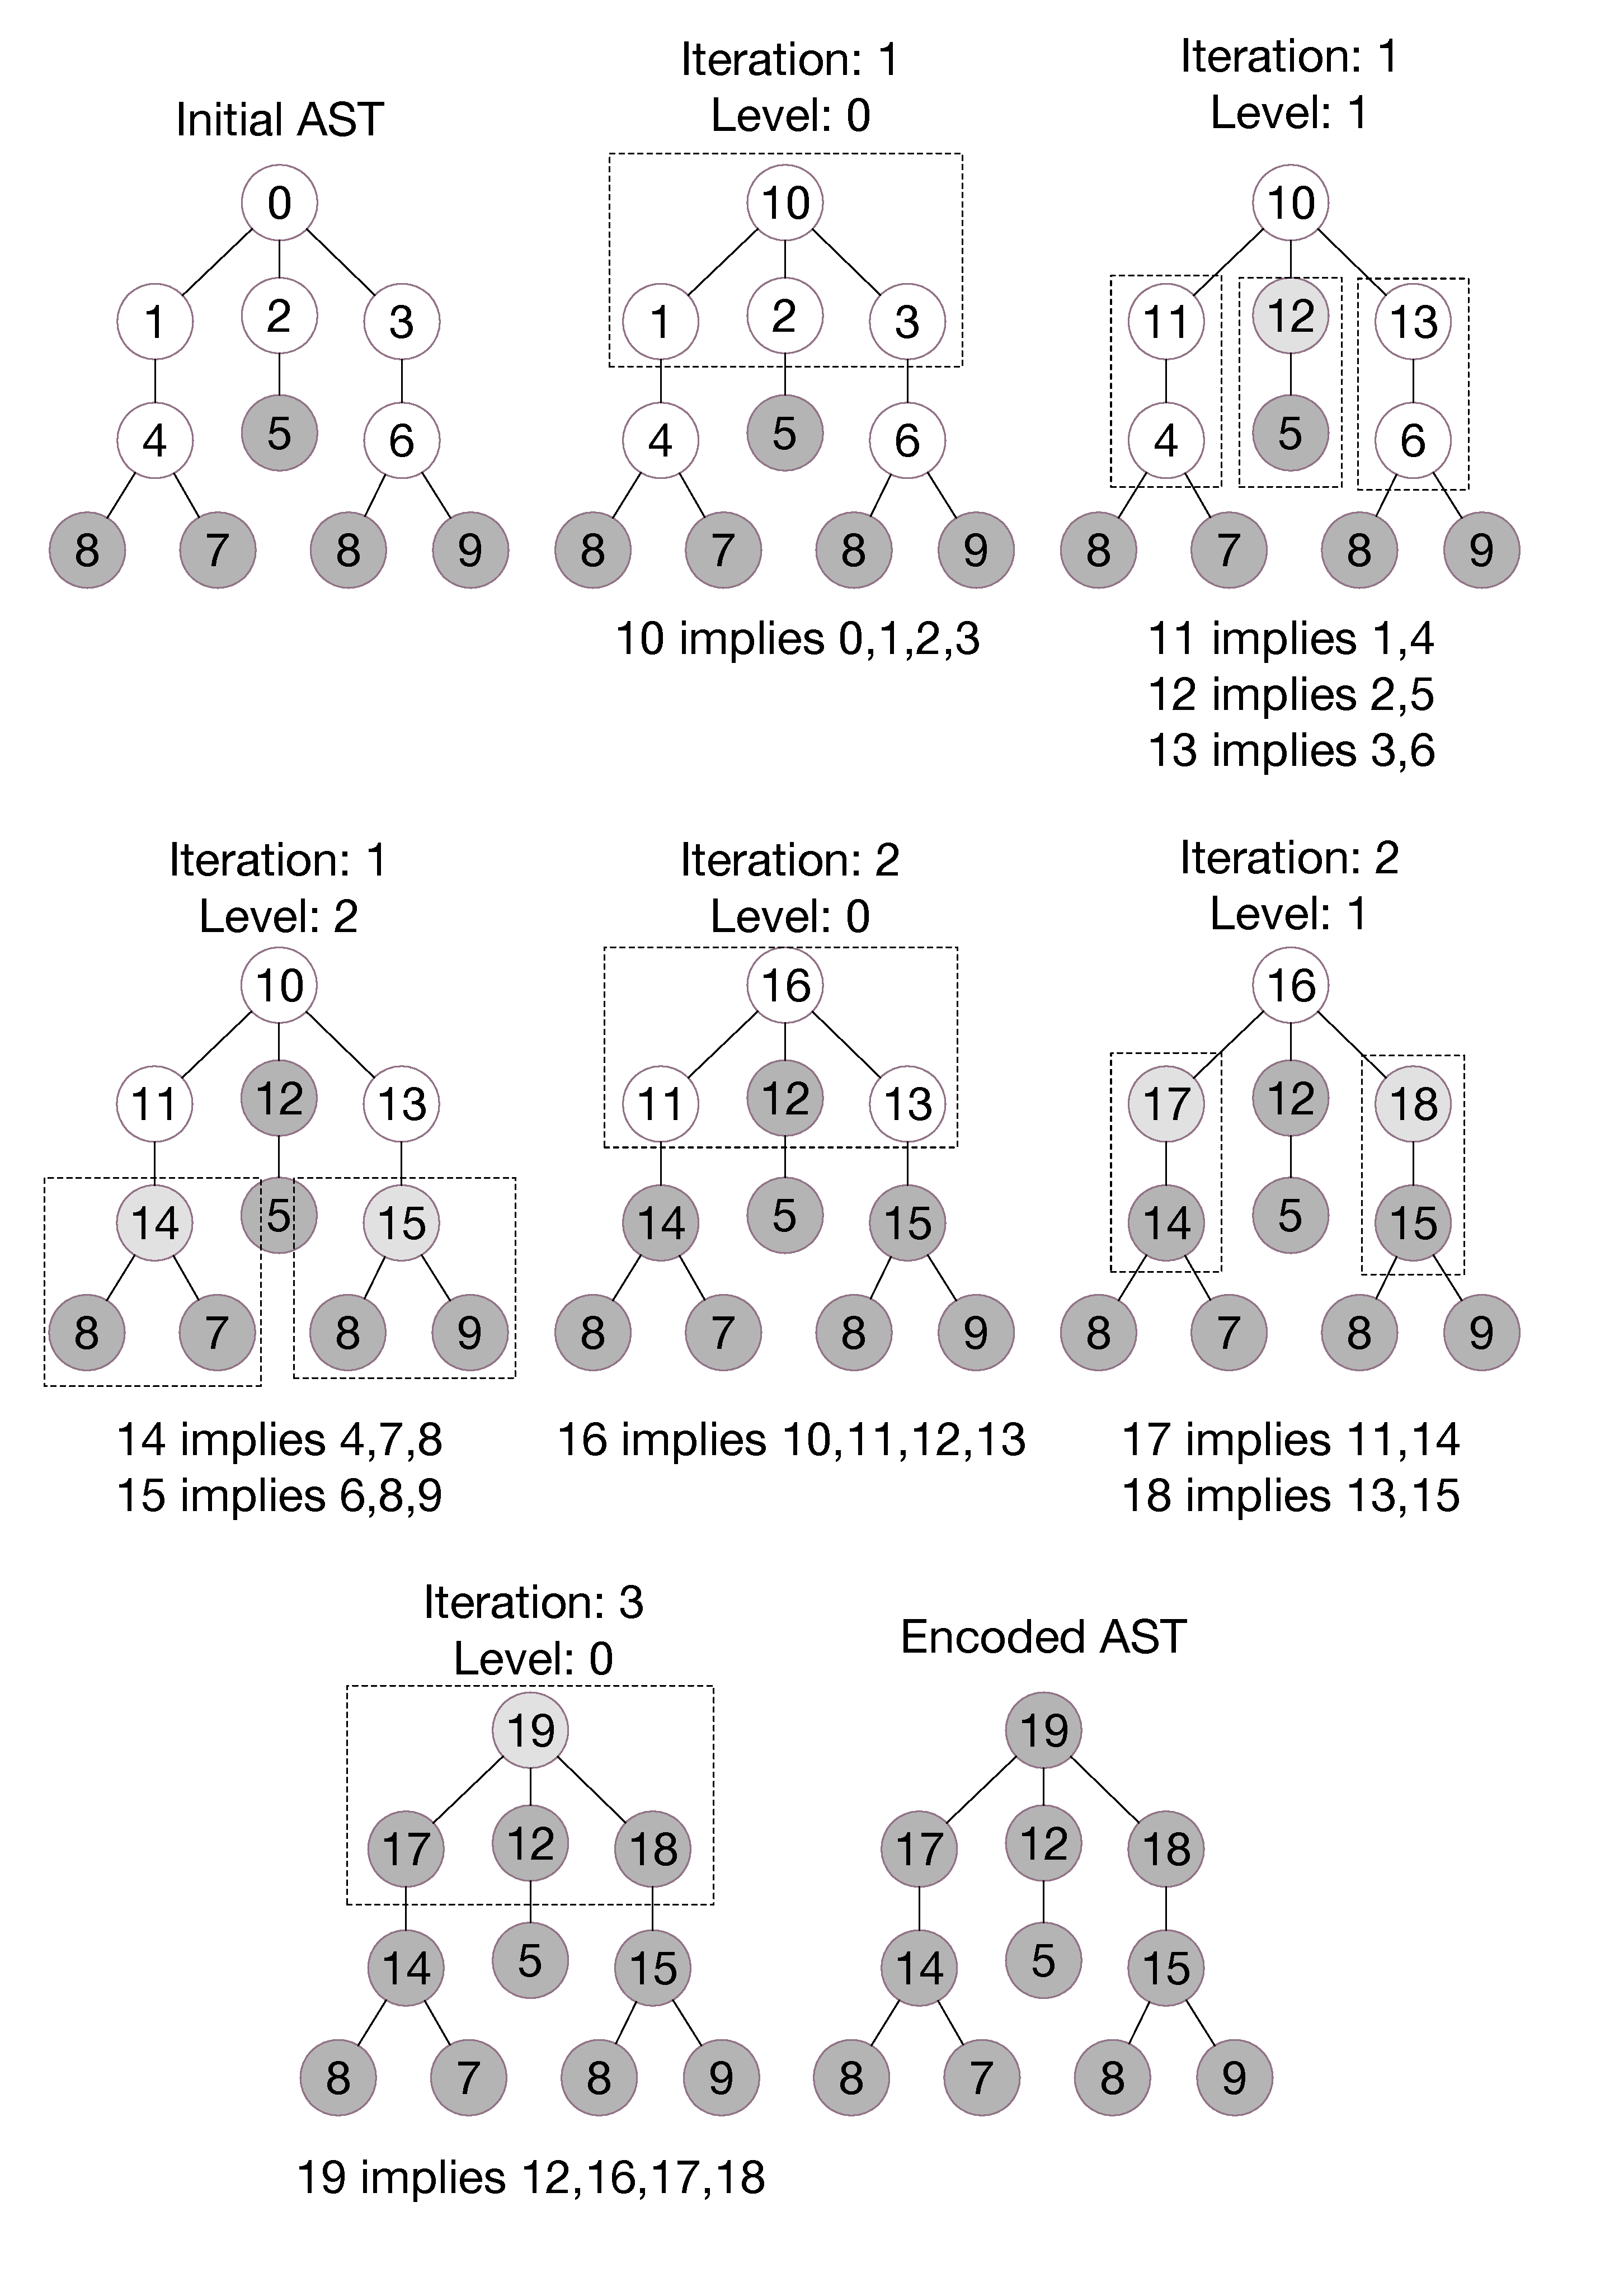
\includegraphics[width=\columnwidth]{graphics/WLExample}
\caption{Weisfeiler-Lehman algorithm applied on AST given in Figure~\ref{fig:exampleAST}.}
\label{fig:wlexample}
\end{figure}

Figure~\ref{fig:wlexample} shows how the WL algorithm is applied on the AST of the query given in Figure~\ref{fig:exampleAST}. First, every distinct node of the AST gets labeled with a unique integer.  If the same node appears more than once, each instance is labeled with the same integer.
As the algorithm progresses, the dotted box emphasizes the region being examined, while the text below represents new labels being synthesized from existing labels.  Grey nodes have been fully labeled, while white nodes are still being processed.

\begin{figure*}[h!]
	\captionsetup[subfigure]{justification=centering}
    \centering
    \begin{subfigure}[b]{0.3\textwidth}
        \centering
        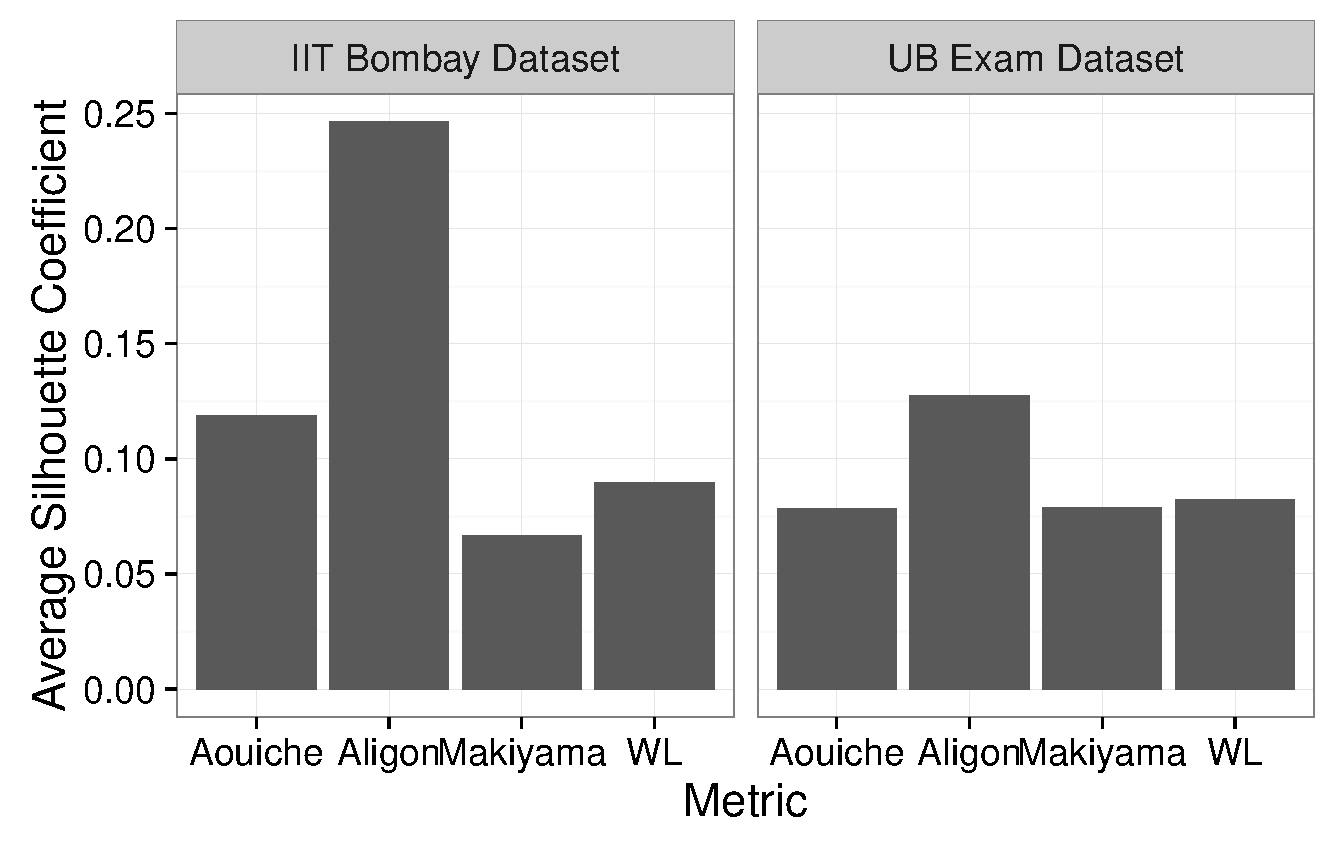
\includegraphics[width=\textwidth]{graphics/silhouette3}
        \caption{Average Silhouette Coefficient\\(the larger value is better)}
    \end{subfigure}%
    ~
    \begin{subfigure}[b]{0.3\textwidth}
        \centering
        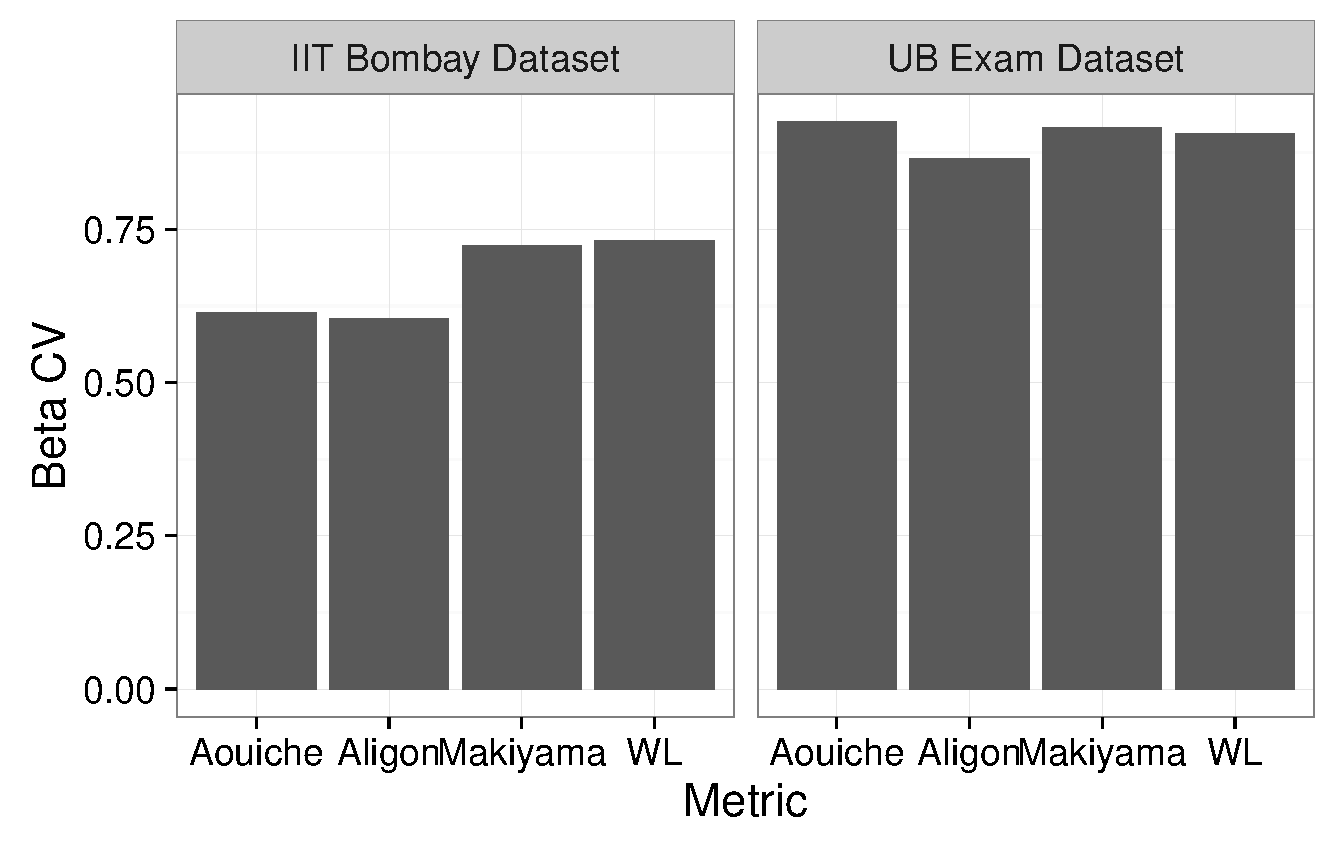
\includegraphics[width=\textwidth]{graphics/beta_cv3}
        \caption{BetaCV\\(the smaller value is better)}
    \end{subfigure}
    ~
    \begin{subfigure}[b]{0.3\textwidth}
        \centering
        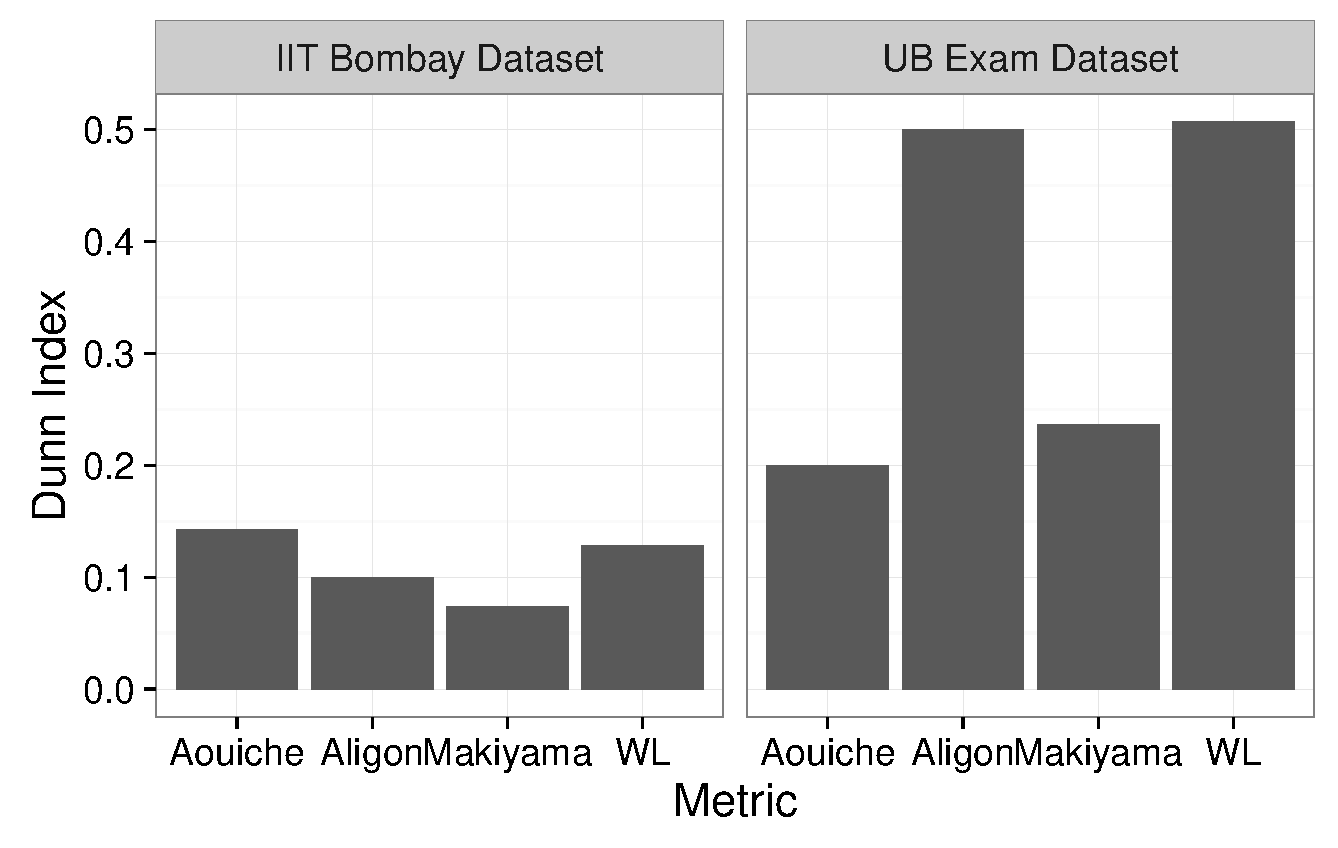
\includegraphics[width=\textwidth]{graphics/dunn3}
        \caption{Dunn Index\\(the larger value is better)}
    \end{subfigure}
    \caption{Comparing the performance of WL algorithm with other similarity metrics}
    \label{fig:comparison3}
\end{figure*}

\begin{figure*}[h!]
	\captionsetup[subfigure]{justification=centering}
    \centering
    \begin{subfigure}[b]{0.3\textwidth}
        \centering
        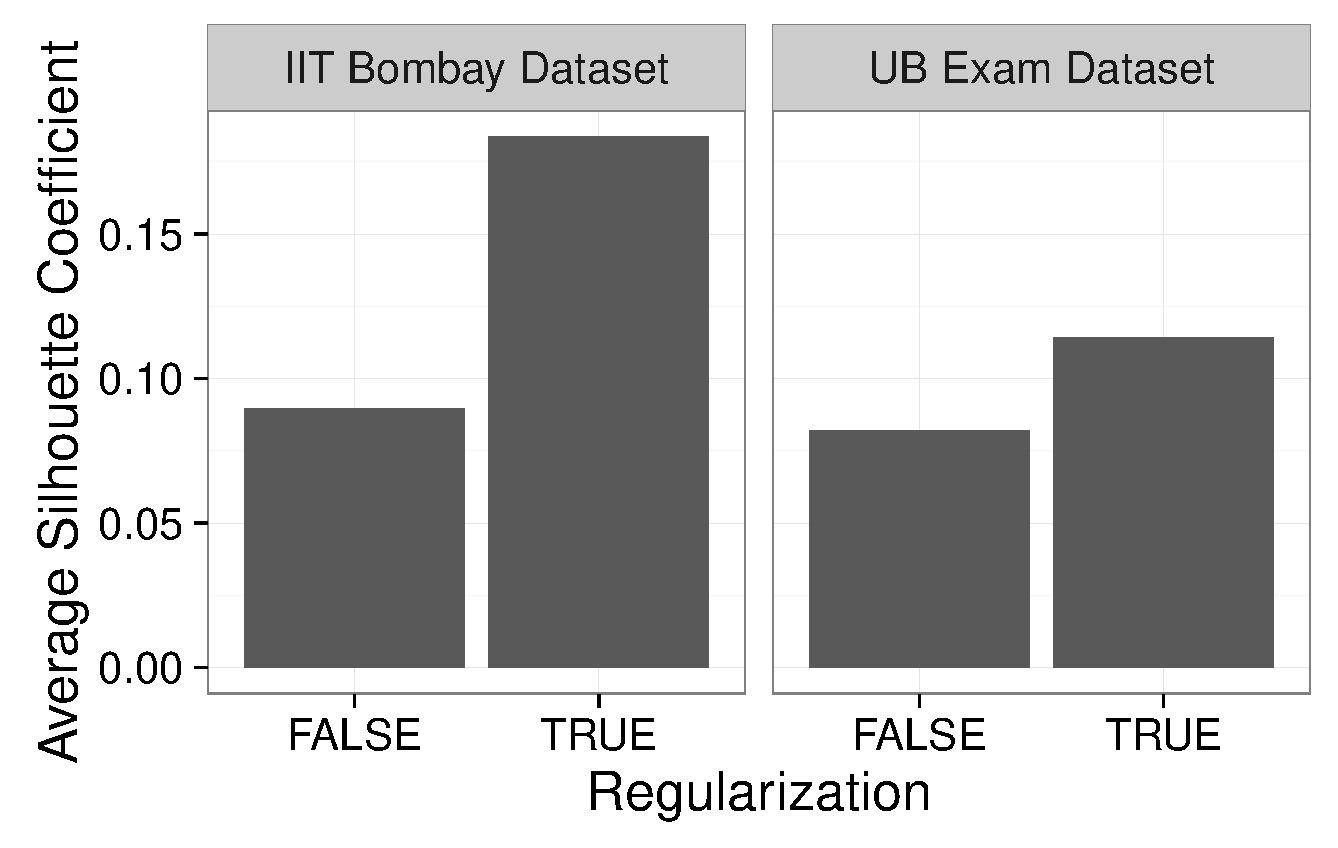
\includegraphics[width=\textwidth]{graphics/silhouette4}
        \caption{Average Silhouette Coefficient\\(the larger value is better)}
    \end{subfigure}%
    ~
    \begin{subfigure}[b]{0.3\textwidth}
        \centering
        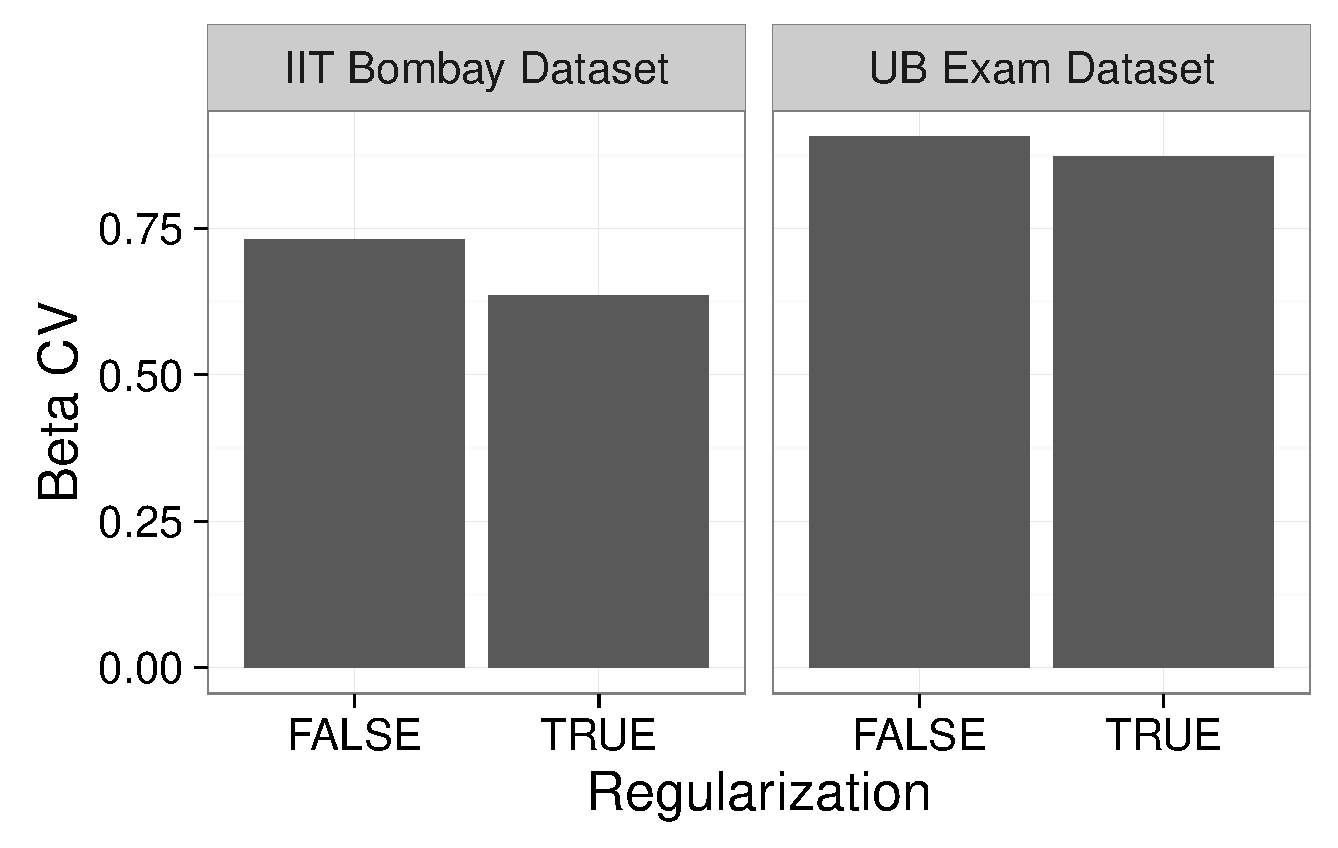
\includegraphics[width=\textwidth]{graphics/beta_cv4}
        \caption{BetaCV\\(the smaller value is better)}
    \end{subfigure}
    ~
    \begin{subfigure}[b]{0.3\textwidth}
        \centering
        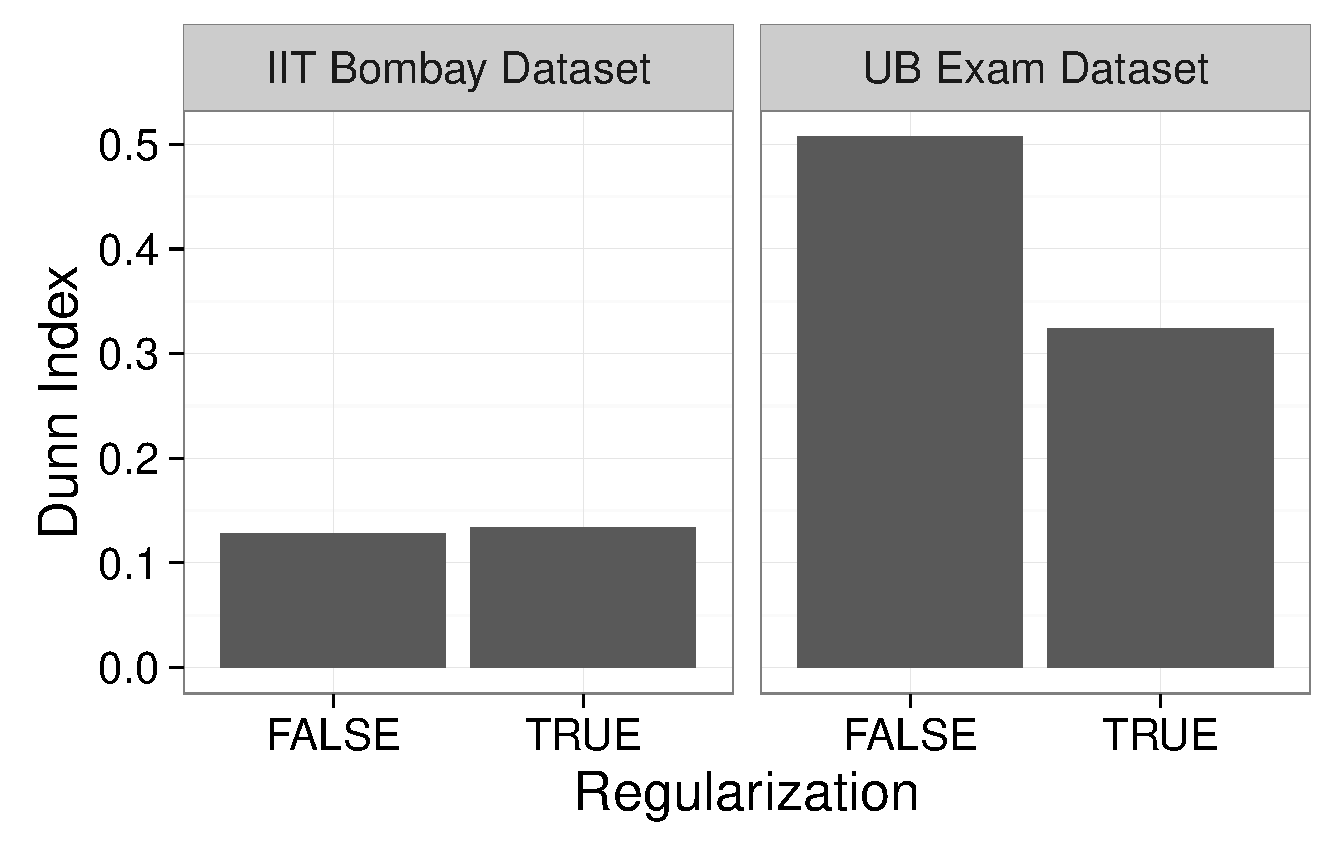
\includegraphics[width=\textwidth]{graphics/dunn4}
        \caption{Dunn Index\\(the larger value is better)}
    \end{subfigure}
    \caption{Comparing performance of WL algorithm with and without regularization step}
    \label{fig:comparison4}
\end{figure*}

\subsection{Clustering using the similarity metric} 

%The next step is to cluster queries by their feature vectors. The result of this process is a set of clusters in which queries with similar structures are grouped together. We considered two possible clustering approaches for use: k-means and hierarchical clustering~\cite{xu2005survey}.
%K-means outputs a set of query skeletons for \textit{k} clusters. 
%On the other hand, hierarchical clustering outputs a dendrogram -- a tree structure which shows how each query can be grouped together.
%For our specific use case where we aim to summarize groups of similar queries, the number of groups or clusters is not known in advance. For this reason, we eventually elected to use hierarchical clustering because it gives us the flexibility to choose the number of clusters after computing the dendrogram. 
%In addition, a dendrogram is a convenient way to visualize the relationship between queries and how each query is grouped in the clustering process. 

%Hierarchical clustering recursively selects the closest pair of data points and merges them into a single virtual data point.  This process requires an agglomerative rule, a formula for aggregating feature vectors together into the vector of each virtual data point.
%There are several often used possibilities, including complete--linkage, single--linkage and average--linkage.
%In our experiments, the choice of agglomerative rules does not significantly change the clustering result; all commonly used agglomerative rules produce equally reliable outputs.
%Consequently, we arbitrarily chose to use complete--linkage, in which the farthest distance from a data point in one cluster to a data point in another cluster is considered as the distance between two clusters. 

%Another aspect that we should consider when doing hierarchical clustering is the distance metric to compare a pair of data points. 
%Since every query skeleton is represented as a feature vector, we have to determine distance metric for computing distance between two feature vectors. 
In our experiments, we use cosine similarity as the similarity metric. We could have used Euclidean or Manhattan distance, too, but in that case we would need to have an additional normalization step; for instance, when we compare two queries with only one feature different from each other, our result would be 2 units. However, when we compare two queries with hundreds of features in common, but only three features different, our result would be 3 units, hence we would classify the latter pair more different than the former pair. We can perform clustering of similar queries with the pairwise similarity matrix of a query set by creating the feature vectors with WL algorithm, and then calculating pairwise distances with cosine similarity.

The accuracy of this method to extract important features can be increased in various ways. In Section~\ref{sec:system}, we talk about how we can exploit the flexibility of SQL queries by regularization. We also discuss what can be done to improve the algorithm's performance in Section~\ref{sec:discussion}. In the following section, we show how this similarity metric compares against the other similarity metrics evaluated in this paper.

\subsection{Evaluation}

In order to evaluate our the effectiveness of WL algorithm in characterize query similarity, we compare it against three other metrics which have been mentioned in Section~\ref{sec:experiments}. Figure~\ref{fig:comparison3} shows the comparison of all four metrics using three different clustering validation measures. We, again, use the UB Exam dataset with the queries graded over 50\% and IIT Bombay dataset for the same reasons explained in Section~\ref{subsec:evaluation}. As observed in the figure, even though WL algorithm is not the best across three different measures, it is quite competitive in comparison with other similarity metrics. This shows WL algorithm has a great potential for improvement when it is only used in its straightforward form and hasn't been tweaked much to adapt with the query data. 

Beside it, we also want to explore how well WL algorithm works when using regularization step. For this reason, we perform another experiment to compare the effectiveness of WL algorithm with and without regularization step. Figure~\ref{fig:comparison4} shows the result of this experiment. As observed in the figure, adding regularization step can yield an improvement in performance of WL algorithm when considering Average Silhouette Coefficient or BetaCV as a quality measure. On the other hand, there is no clear improvement or even a reduction in clustering quality when Dunn Index is used as a clustering validation measure. However, the same argument from subsection~\ref{subsec:evaluation} can be applied here when noting that Dunn Index only measures the extreme cases in the dataset while Average Silhouette Coefficient and BetaCV consider all queries in dataset when computing the measures. Therefore, we may conclude that even though some queries at the borderline of cluster may suffer a decrease in clustering quality, adding regularization step into WL algorithm will increase in its overall capability of capturing query semantics and put queries that perform the same task spatially close together.

For understanding the computational time to process a set of queries and producing pair-wise distance matrix for WL algorithm and its relative processing time to other similarity metrics, we measure and report the running time of each similarity metric with and without regularization. For all metrics, the running time is measured 5 times and the average value is reported. Figure~\ref{fig:running_time} shows the comparison in terms of running time among different similarity metrics. As observed in the figure, when using regularization, the running time is consistently reduced except for the case of Makiyama's similarity metric when IIT Bombay dataset is used. For UB Exam dataset, probably because of the small number of queries, the running time is almost comparable among four similarity metrics. With IIT Bombay dataset where the number of queries is nearly three times more than the number of queries in UB Exam dataset, the difference in running among different similarity metrics are more notable. Although WL algorithm is slowest among four metrics when regularization step doesn't apply, its running time decreases drastically when using regularization. This can be explained by noting that the regularization step allows the query to be converted into a more standardized form which subsequently is more efficient in extracting features and leads to a reduction in running time.

\begin{figure}[h!]
	\centering
    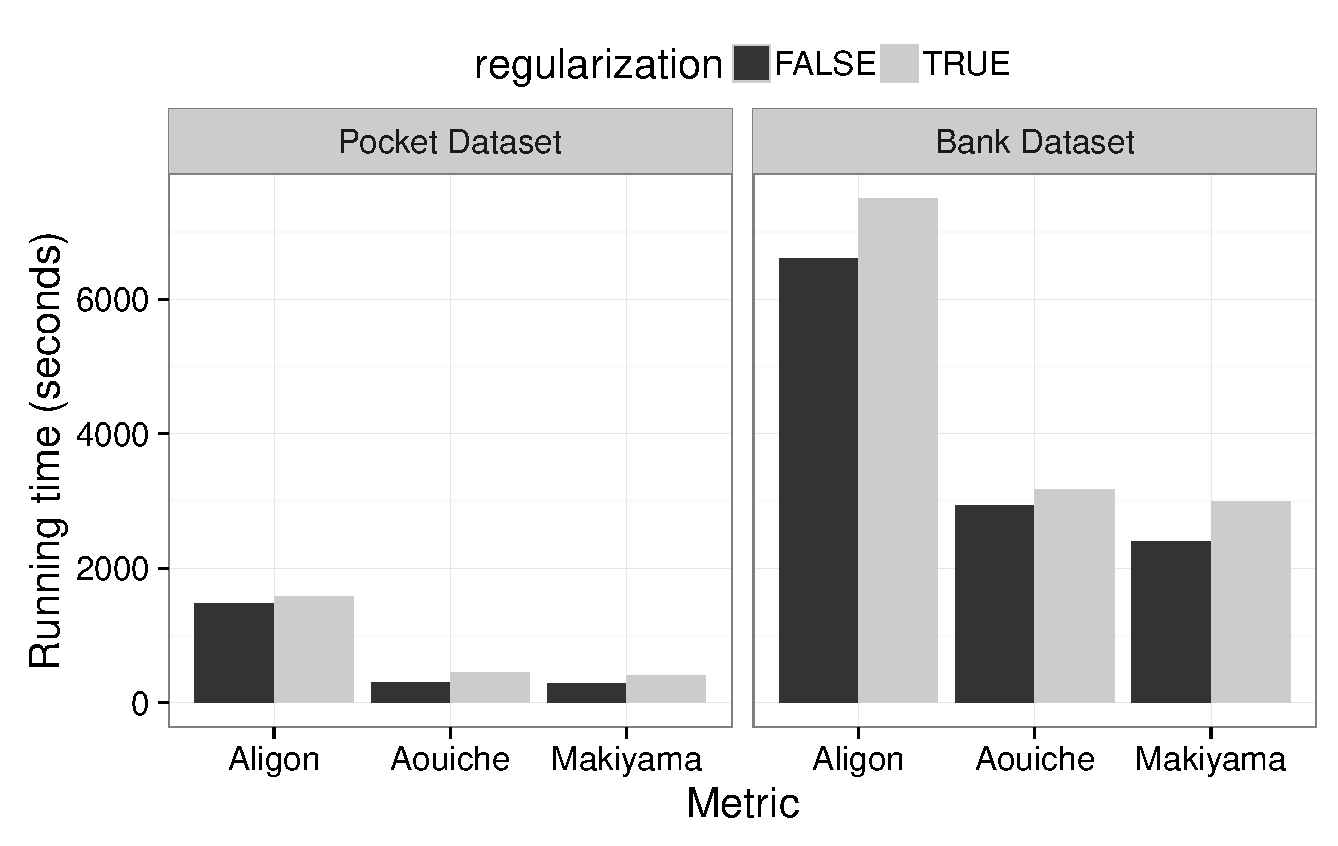
\includegraphics[width=0.5\textwidth]{graphics/running_time}
    \caption{Running time comparison among different query similarity metrics with and without regularization}
    \label{fig:running_time}
\end{figure}